\section{Introduction}

\begin{frame}[<+->]{Introduction - Heavy Quarks}
HQ are good
\end{frame}

\begin{frame}[<+->]{Introduction - Experimental Setups}
\begin{center}
\newcolumntype{C}{>{\centering\arraybackslash} m{3.6cm} } 
\begin{tabular}{C|C|C}
\Pelectron-\APelectron-annihilation (SIA) & deep inelastic scattering (DIS) & Drell-Yan process (DY)\\
%SIA & DIS & DY\\
\hline
$\Pelectron+\APelectron \rightarrow \PaQ + X[\PQ]$ &
$\Pl+h \rightarrow \PaQ + X[\PQ]$ &
$h + h' \rightarrow \PaQ + X[\PQ]$ \\
\hline
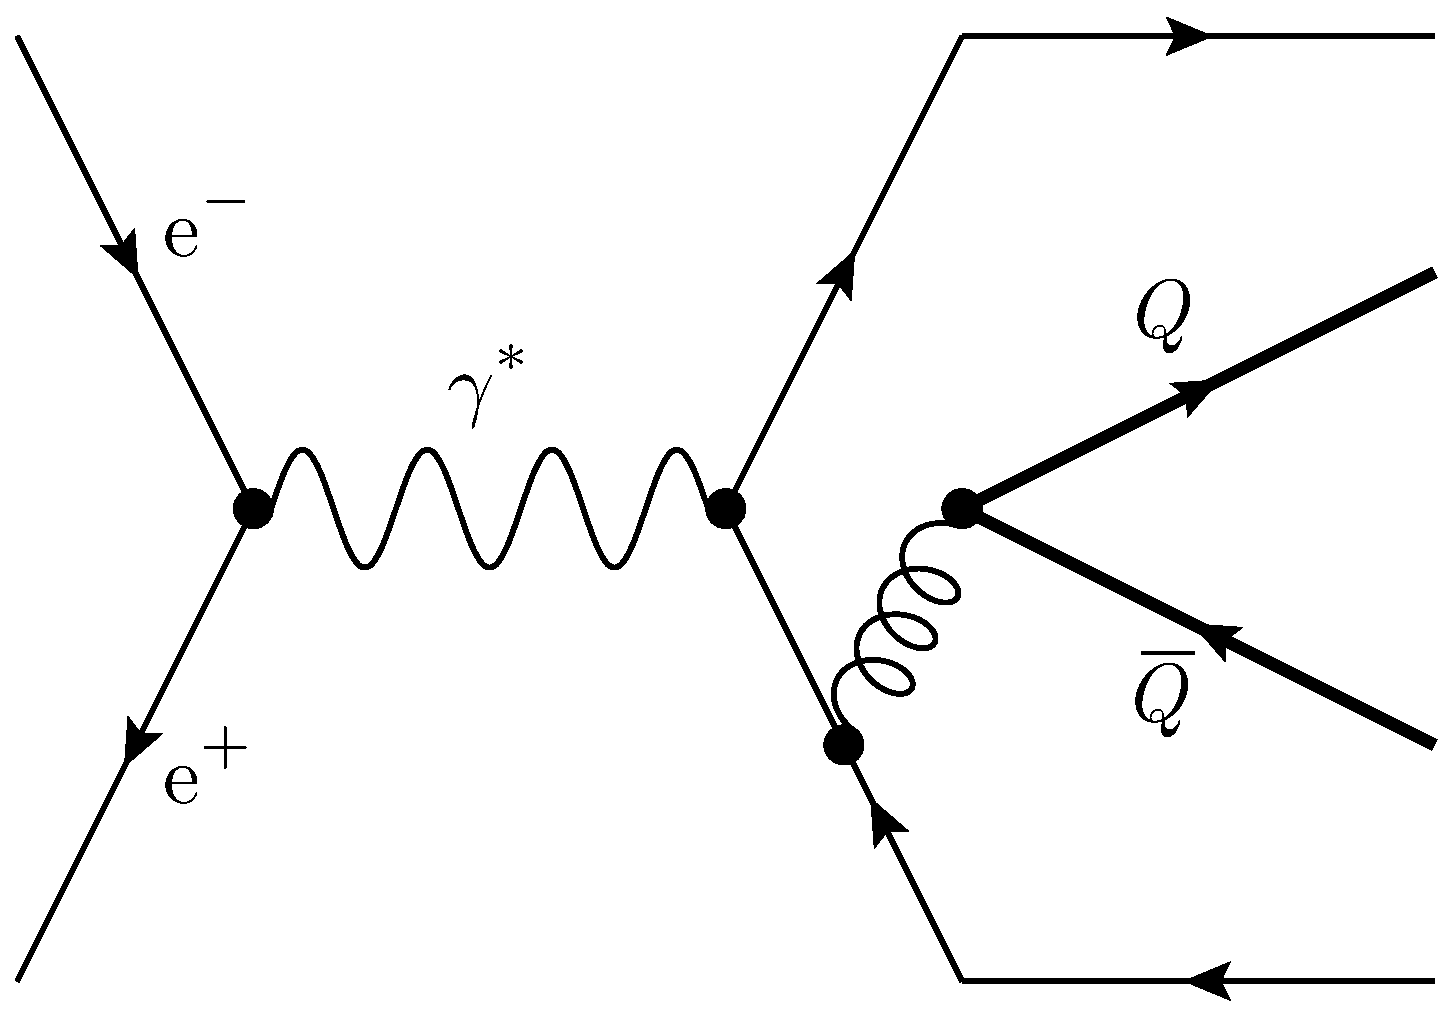
\includegraphics[width=.25\textwidth]{img/SIA.eps} & 
\vspace{.2cm}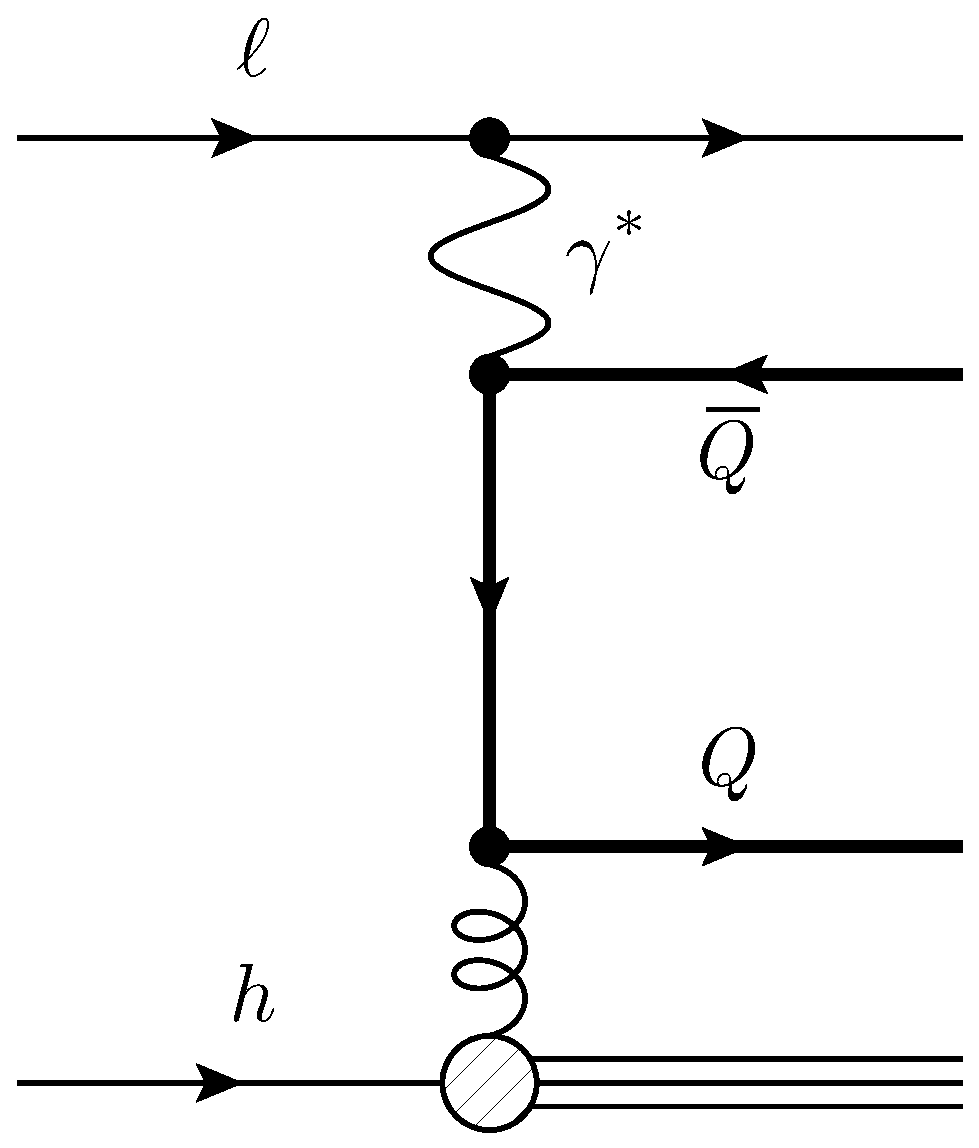
\includegraphics[width=.25\textwidth]{img/DIS.eps} & 
\vspace{.2cm}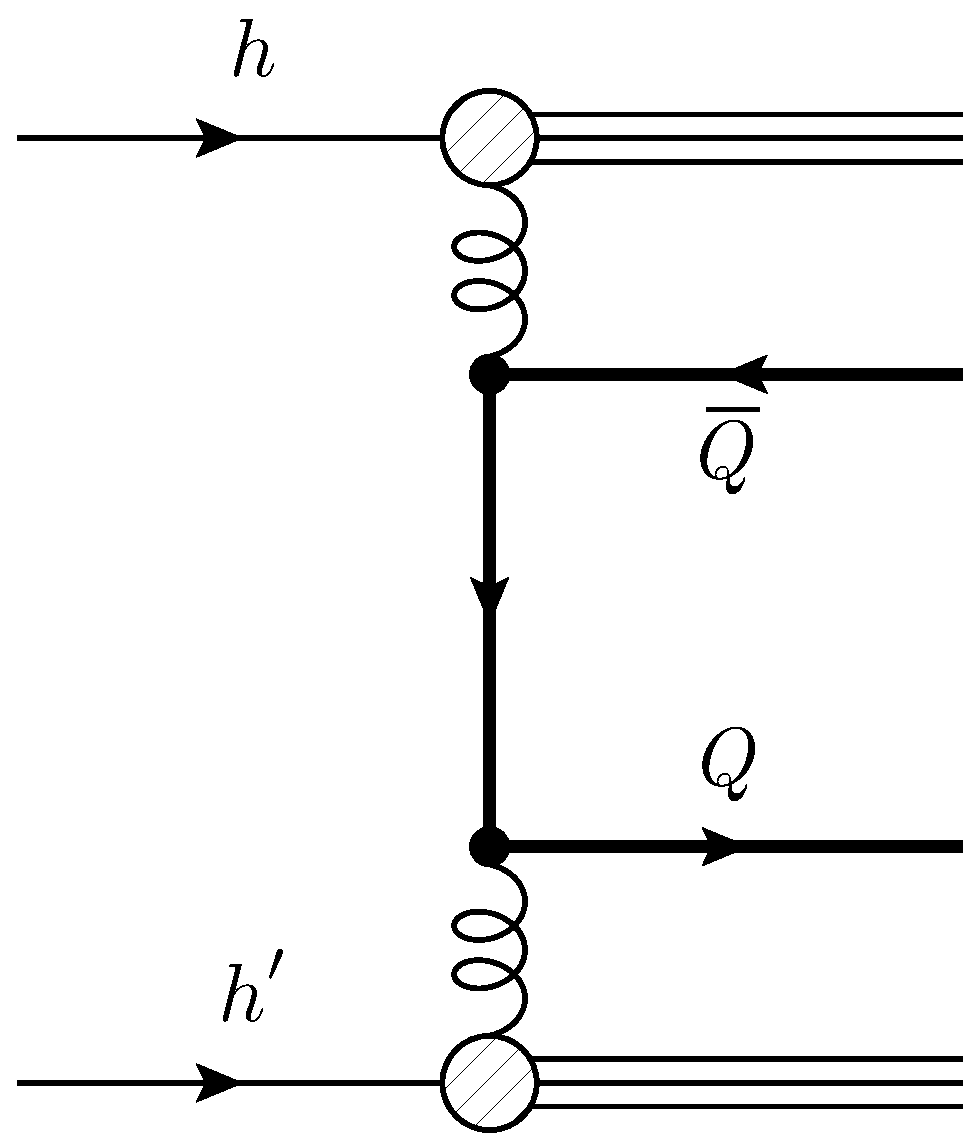
\includegraphics[width=.25\textwidth]{img/DY.eps} \\
\hline
LEP, ILC & HERA, COMPASS, EIC & Tevatron, LHC\\
\hline
gluon & factorization & top, Higgs
\end{tabular}
\end{center}
\end{frame}

\begin{frame}[<+->]{Introduction - Structure Functions}
\begin{align}
&&\frac{d^2\sigma}{dx dy} &= \frac{2\pi y \alpha^2}{Q^4} L^{\mu\nu} W_{\mu\nu}\\
&\text{hard. tensor:}&W_{\mu\nu} &= \left(-g_{\mu\nu} + \frac{q_\mu q_\nu}{q^2}\right) F_1(x,Q^2) + \frac{P_\mu P_\nu}{P\cdot q} F_2(x,Q^2) \nonumber\\
&& & \hspace{20pt} + i \epsilon_{\mu\nu\alpha\beta} \frac{q^{\alpha}S^{\beta}}{P\cdot q} g_1(x,Q^2)\\
&&F_L(x,Q^2) &= F_2(x,Q^2) - 2xF_1(x,Q^2)\\
&\text{unpol. cs:}&\frac{d^2\sigma}{dx dy} &= \frac{2\pi \alpha^2}{x y Q^2}\left(Y_+F_2(x,Q^2) - y^2F_L(x,Q^2)\right)\\
&\text{pol. cs:}&\frac{d^2\Delta\sigma}{dx dy} &= \frac{4\pi \alpha^2}{x y Q^2}Y_-\cdot 2xg_1(x,Q^2)\\
&&Y_\pm &= 1 \pm (1-y)^2
\end{align}
\end{frame}
